\begin{prop}
\[
\norme{\Pi^\surflisse_\ensddfv u^\ensddfv}^2_{\L^2(\surflisse)} \sim h^2 \sum_{\primal{K} \in \ensprimal} u_{\primal{K}}{}^2
\]
\end{prop}

\begin{prop}
\[
\normeddfvD{} \sim \norme{}_{\L^2(\surflisse)}   
\]
\end{prop}

\begin{prop}
\begin{equation}
\underline{C}^\ensddfv \leqslant \norme{\projddfvvar}_{\L^2} \leqslant \overline{C}^\ensddfv,
\quad
\underline{C}^\ensdiamant \leqslant \norme{\projdiamantvar}_{\L^2} \leqslant \overline{C}^\ensdiamant.
\end{equation}
\end{prop}

\begin{demo}
\[
\norme{\projddfvvar}_{\L^2} = \sup_{u^\ensddfv \in \R^\ensddfv} \frac{\norme{\projddfvvar u^\ensddfv}_{\L^2(\surflisse)}}{\normeddfvT{u^\ensddfv}}
\]
\end{demo}

\begin{corol}
On a
\[
\norme{\projddfvvar u^\ensddfv}_{\L^2(\surflisse)} \leqslant C \, \frac{\overline{C}^\ensdiamant}{\underline{C}^\ensddfv} \norme{\projdiamantvar \grad^\ensdiamant u^\ensddfv}_{\L^2(\surflisse)}.
\]
\end{corol}


\areprendre{
For any function $\eta$ defined on the discrete surface $\surfpoly$ we define an extension or lift onto $\surflisse$ by
\begin{equation} \label{eq:lift}
\eta^\ell(a) = \eta(x(a)), \quad a \in \surflisse,    
\end{equation}
where, by our assumptions, $x(a)$ is defined as the unique solution of
\[
x = a + d(x) \, \nu(a).
\]
Furthermore, we understand by $\eta^\ell(x)$ the constant extension from $\surflisse$ in the normal direction $\nu(a(x))$.

In order to compare the norms between functions on $\surfpoly$ and their lift \ref{eq:lift} to $\surflisse$ we need the following lemma. 

\begin{lemme}
Let $\fonctionens[\eta]{\surfpoly}{\R}$ with the lift $\fonctionens[\eta^\ell]{\surflisse}{\R}$. Then, for the plane $T \subset \surfpoly$, and smooth curved triangles $\widetilde{T} \subset \surflisse$, the following estimates hold is the norm exist. There is a constant $c > 0$ independant of $h$ such that
\begin{align*}
    \frac{1}{c} \norme{\eta}_{\L^2(T)} &\leqslant \norme{\eta^\ell}_{\L^2(\widetilde{T})} \leqslant c \norme{\eta}_{\L^2(T)}, \\
    \frac{1}{c} \norme{\grad_{\surfpoly} \eta}_{\L^2(T)} &\leqslant \norme{\grad_{\surflisse} \eta^\ell}_{\L^2(\widetilde{T})} \leqslant c \norme{\grad_{\surfpoly} \eta}_{\L^2(T)}, \\
    \norme{\grad^2_{\surfpoly} \eta}_{\L^2(T)} &\leqslant c \norme{\grad^2_{\surflisse} \eta^\ell}_{\L^2(\widetilde{T})} + c \, h \norme{\grad_{\surflisse} \eta^\ell}_{\L^2(\widetilde{T})}.
\end{align*}
\end{lemme}
}

\begin{figure}
\[
\begin{tikzcd}
\mathrm{scal.} & \mathrm{vect.} & \mathrm{scal.} \\
\Lambda^0 
\arrow[r,rightarrow, yshift=0.4ex, "\grad"] \arrow[r,leftarrow, yshift=-0.4ex, "\div"'] 
& 
\Lambda^1
\arrow[r,rightarrow, yshift=0.4ex, "\rot"] \arrow[r,leftarrow, yshift=-0.4ex, "\grad^\perp"']
&
\Lambda^2
\end{tikzcd}
\]
\caption{}
\end{figure}


\begin{figure}[H]
\centering
\begin{subfigure}[t]{.5\textwidth}
    \centering
    \input{figures/duality_div_grad.tex}
    \caption{}
\end{subfigure}%
\begin{subfigure}[t]{.5\textwidth}
    \centering
    \begin{tikzpicture}[scale=2]
    \node (A) at (0,0) {$\R^\ensddfv$};
    \node (B) at (1,0) {$(\R^2)^\ensdiamant$};

    \draw[->] (A) to [bend left=25] node[midway, above] {$\rot^\ensdiamant$} (B);
    \draw[->] (B) to [bend left=25] node[midway, below] {$\scarot^\ensddfv$} (A);
\end{tikzpicture}
    \caption{}
\end{subfigure}
\caption{}
\end{figure}

\begin{figure}[H]
    \centering
    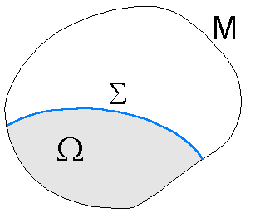
\includegraphics[width=0.3\textwidth]{img/isoperimetric-problem-in-a-region.png}
    \caption{}
\end{figure}

\begin{prop}
\areprendre{
L'opérateur divergence discrète peut s'écrire sous la forme $\fonctionens[\div^\ensddfvplat]{(\R^2)^\ensdiamantplat}{\R^\ensddfvplat}$. Soit $\xi^\ensdiamantplat \in (\R^2)^\ensdiamantplat$, on pose
\[
\div^\ensddfvplat \xi^\ensdiamantplat = \mathopen{}\big( 
\div^\ensprimalplat \xi^\ensdiamantplat,
\div^\ensdualplat \xi^\ensdiamantplat    
\big),
\]
avec $\div^\ensprimalplat \xi^\ensdiamantplat = \mathopen{}\big(\div^{\primalplat{K}} \xi^\ensdiamantplat \big)_{\primalplat{K} \in \ensprimalplat}$, $\div^\ensdualplat \xi^\ensdiamantplat = \mathopen{}\big( \div^{\mailledualeplate{K}} \xi^\ensdiamantplat \big)_{\mailledualeplate{K} \in \ensdualplat}$:
\begin{align*}
    \forall \primalplat{K} \in \ensprimalplat, \quad \div^{\primalplat{K}} \xi^\ensdiamantplat &= \frac{1}{\mesure(\primalplat{K})} \sum_{\diamantplat{D}_{\sigma, \dual{\sigma}} \in \ensdiamantplat_{\primalplat{K}}} \mesure(\sigma) \, \xi^{\diamantplat{D}} \cdot \vect{\nu}, \\
    \forall \mailledualeplate{K} \in \ensdualplat, \quad \div^{\mailledualeplate{K}} \xi^\ensdiamantplat &= \frac{1}{\mesure(\mailledualeplate{K})} \sum_{\diamantplat{D}_{\sigma, \dual{\sigma}} \in \ensdiamantplat_{\mailledualeplate{K}}} \mesure(\dual{\sigma}) \, \xi^{\diamantplat{D}} \cdot \dual{\vect{\nu}}.
\end{align*}    
}
\end{prop}

% % Démonstration de la formule locale de la divergence discrète.
% Ce fichier peut être inclus à la place de l'environnement `demo` vide.

Soit $u^\ensddfvplat \in \R^\ensddfvplat$. Par définition de la
divergence discrète comme opposé de l'adjoint du gradient,
\begin{equation}\label{eq:preuve_div_adjonction}
    \prodscalddfv{u^\ensddfvplat}{\div^\ensddfvplat\xi^\ensdiamantplat}
    =-
    \prodscalD{\grad^\ensdiamantplat u^\ensddfvplat}{\xi^\ensdiamantplat}.
\end{equation}
Développons le membre de droite diamant par diamant. Pour
$\diamantplat{D}_{\sigma,\dual{\sigma}}$, la formule du gradient donne
\[
\grad^{\diamantplat{D}}u^\ensddfvplat
=\frac{1}{\sin\angle{\diamantplat{D}}}
\left(
 \frac{u_{\primalplat{L}}-u_{\primalplat{K}}}{\mesure(\dual{\sigma})}
 \vect{\nu}_{\sigma\primalplat{K}}
 +
 \frac{u_{\mailledualeplate{L}}-u_{\mailledualeplate{K}}}{\mesure(\sigma)}
 \vect{\nu}_{\dual{\sigma}\mailledualeplate{K}}
\right).
\]
Or
\[
\mesure(\diamantplat{D})
=\frac12\mesure(\sigma)\mesure(\dual{\sigma})
 \sin\angle{\diamantplat{D}}.
\]
Par conséquent,
\begin{align*}
-\prodscalD{\grad^\ensdiamantplat u^\ensddfvplat}{\xi^\ensdiamantplat}
={}&-\frac12\sum_{\diamantplat{D}_{\sigma,\dual{\sigma}}\in\ensdiamantplat}
 \mesure(\sigma)
 (u_{\primalplat{L}}-u_{\primalplat{K}})
 \xi^{\diamantplat{D}}\cdot\vect{\nu}_{\sigma\primalplat{K}}
\\
&-\frac12\sum_{\diamantplat{D}_{\sigma,\dual{\sigma}}\in\ensdiamantplat}
 \mesure(\dual{\sigma})
 (u_{\mailledualeplate{L}}-u_{\mailledualeplate{K}})
 \xi^{\diamantplat{D}}\cdot
 \vect{\nu}_{\dual{\sigma}\mailledualeplate{K}}.
\end{align*}

Regroupons maintenant les termes qui multiplient une même valeur
$u_{\primalplat{K}}$. Sur une arête $\sigma$ de $\primalplat{K}$, la
normale $\vect{\nu}_{\sigma\primalplat{K}}$ est la normale extérieure à
$\primalplat{K}$. Si $\primalplat{K}$ est désignée comme la seconde
maille du diamant, l'inversion simultanée de la différence des valeurs
et de la normale donne le même terme. Le coefficient de
$u_{\primalplat{K}}$ dans le membre de droite de
\eqref{eq:preuve_div_adjonction} est donc
\[
\frac12
\sum_{\diamantplat{D}_{\sigma,\dual{\sigma}}
      \in\ensdiamantplat_{\primalplat{K}}}
\mesure(\sigma)\,
\xi^{\diamantplat{D}}\cdot\vect{\nu}_{\sigma\primalplat{K}}.
\]
De même, le coefficient de $u_{\mailledualeplate{K}}$ vaut
\[
\frac12
\sum_{\diamantplat{D}_{\sigma,\dual{\sigma}}
      \in\ensdiamantplat_{\mailledualeplate{K}}}
\mesure(\dual{\sigma})\,
\xi^{\diamantplat{D}}\cdot
\vect{\nu}_{\dual{\sigma}\mailledualeplate{K}}.
\]

D'autre part, puisque
$\poids{\primalplat{K}}=\mesure(\primalplat{K})/2$ et
$\poids{\mailledualeplate{K}}=\mesure(\mailledualeplate{K})/2$, le
membre de gauche de \eqref{eq:preuve_div_adjonction} est
\begin{align*}
&\frac12\sum_{\primalplat{K}\in\ensprimalplat}
 \mesure(\primalplat{K})u_{\primalplat{K}}
 \div^{\primalplat{K}}\xi^\ensdiamantplat
\\
&\qquad+
\frac12\sum_{\mailledualeplate{K}\in\ensdualplat}
 \mesure(\mailledualeplate{K})u_{\mailledualeplate{K}}
 \div^{\mailledualeplate{K}}\xi^\ensdiamantplat.
\end{align*}
L'identité étant vraie pour tout $u^\ensddfvplat$, l'identification des
coefficients de ses composantes fournit
\[
\div^{\primalplat{K}}\xi^\ensdiamantplat
=\frac{1}{\mesure(\primalplat{K})}
 \sum_{\diamantplat{D}_{\sigma,\dual{\sigma}}
       \in\ensdiamantplat_{\primalplat{K}}}
 \mesure(\sigma)\,
 \xi^{\diamantplat{D}}\cdot\vect{\nu}_{\sigma\primalplat{K}},
\]
et
\[
\div^{\mailledualeplate{K}}\xi^\ensdiamantplat
=\frac{1}{\mesure(\mailledualeplate{K})}
 \sum_{\diamantplat{D}_{\sigma,\dual{\sigma}}
       \in\ensdiamantplat_{\mailledualeplate{K}}}
 \mesure(\dual{\sigma})\,
 \xi^{\diamantplat{D}}\cdot
 \vect{\nu}_{\dual{\sigma}\mailledualeplate{K}},
\]
ce qui est précisément le résultat annoncé.


\begin{prop}
\areprendre{
$\fonctionens[\scarot^\ensddfvplat]{(\R^2)^\ensdiamantplat}{\R^\ensddfvplat}$. Soit $\xi^\ensdiamantplat \in (\R^2)^\ensdiamantplat$, on pose
\[
\scarot^\ensddfvplat \xi^\ensdiamantplat = \mathopen{}\big( 
\scarot^\ensprimalplat \xi^\ensdiamantplat,
\scarot^\ensdualplat \xi^\ensdiamantplat    
\big),
\]
with $\scarot^\ensprimalplat \xi^\ensdiamantplat = \mathopen{}\big(\scarot^{\primalplat{K}} \xi^\ensdiamantplat \big)_{\primalplat{K} \in \ensprimalplat}$, $\scarot^\ensdualplat \xi^\ensdiamantplat = \mathopen{}\big( \scarot^{\mailledualeplate{K}} \xi^\ensdiamantplat \big)_{\mailledualeplate{K} \in \ensdualplat}$:
\begin{align*}
    \forall \primalplat{K} \in \ensprimalplat, \quad \scarot^{\primalplat{K}} \xi^\ensdiamantplat &= \frac{1}{\mesure(\primalplat{K})} \sum_{\diamantplat{D}_{\sigma, \dual{\sigma}} \in \ensdiamantplat_{\primalplat{K}}} \mesure(\sigma) \, \xi^{\diamantplat{D}} \cdot \vect{\tau}, \\
    \forall \mailledualeplate{K} \in \ensdualplat, \quad \scarot^{\mailledualeplate{K}} \xi^\ensdiamantplat &= \frac{1}{\mesure(\mailledualeplate{K})} \sum_{\diamantplat{D}_{\sigma, \dual{\sigma}} \in \ensdiamantplat_{\mailledualeplate{K}}} \mesure(\dual{\sigma}) \, \xi^{\diamantplat{D}} \cdot \dual{\vect{\tau}}.
\end{align*}
}
\end{prop}

\begin{remarque}
La matrice $\rotmat^\top_\ensdiamant \masse_\ensdiamant$ est symétrique positive mais pas définie. Néanmoins, cela n'est pas gênant car la méthode du gradient conjugué converge à un vecteur du noyau de $\gradmat_\ensdiamant$ près. Or le noyau de $\gradmat_\ensdiamant$ contient l'homologie ainsi que des modes hyper-oscillants. De plus, la composante dans le noyau de $\gradmat$ est préservée dans toutes les étapes du gradient conjugué et en prenant comme solution initiale un vecteur nul, cela nous assure de n'obtenir aucun de ces modes tout en convergeant. 
\end{remarque}

Il faudra vérifier que la définition retenue de l'espace harmonique
discret élimine ou identifie éventuellement cette duplication si l'on
souhaite retrouver exactement la dimension topologique continue.


\cite[Sec. 4.3]{delcourte_discrete_2007} In the continuous case, the Hodge decomposition for non simply connected domains reads:
\begin{equation} \label{eq:413}
(\L^2)^2 = \grad V \oplusperp \rot W,
\end{equation}
with $V = \ens[\big]{\phi \in \H^1 \tq \int_\Omega \phi = 0}$ and $W = \ens[\big]{\psi \in \H^1 \tq \cdot}$. To prove an analogous property in the discrete case, we rely on the following result:


A surface embedded in three-dimensional space is closed if and only if it is the boundary of a solid. As with any closed manifold, a surface embedded in Euclidean space that is closed with respect to the inherited Euclidean topology is not necessarily a closed surface; for example, a disk embedded in $\R^3$ that contains its boundary is a surface that is topologically closed but not a closed surface. (\url{https://en.wikipedia.org/wiki/Surface_%28topology%29})


It follows that an orientable closed surface is determined, up to homeomorphism, by its Euler characteristic.


\begin{demo}
La décomposition se ramène donc à un système carré, comportant autant d'équations que d'inconnues. L'existence et l'unicité de la décomposition sont donc équivalentes et nous allons montrer l'unicité par injectivité. On suppose que $\xi^\ensdiamantplat = 0$. En prenant le produit scalaire de \ref{eq:415} avec $\grad^\ensdiamantplat \phi^\ensddfvplat$, on obtient
\[
0 = \normeddfvD{\grad^\ensdiamantplat \phi^\ensddfvplat}^2
+ \prodscalD{\rot^\ensdiamantplat \psi^\ensddfvplat}{\grad^\ensdiamantplat \phi^\ensddfvplat} 
+ \prodscalD{h^\ensdiamantplat}{\grad^\ensdiamantplat \phi^\ensddfvplat}.
\]
Le deuxième terme est nul par le \Cref{theo:rotperpgrad}, ainsi que le troisième en appliquant une formule de Green discrète (voir le \Cref{theo:discrete_green_formulae}) et en utilisant le fait que $h^\ensdiamantplat \in \ker(\div^\ensddfvplat)$. Ainsi, $\grad^\ensdiamantplat \phi^\ensddfvplat = 0$ et comme $\phi^\ensddfvplat \in \Rddfvmn$, on en déduit que $\phi^\ensddfvplat = 0$. De la même manière, en prenant le produit scalaire de \ref{eq:415} avec $\rot^\ensdiamantplat \psi^\ensddfvplat$ et en utilisant que $h^\ensdiamantplat \in \ker(\scarot^\ensddfvplat)$ et que $\psi^\ensddfvplat \in \Rddfvmn$, on obtient que $\psi^\ensddfvplat = 0$. Finalement on obtient $h^\ensdiamantplat = 0$ ce qui fournit l'injectivité et donc l'existence et l'unicité de la décomposition de Helmholtz--Hodge discrète dans le cadre \ddfv.
\end{demo}